\chapter{Descripción general}

\section{Perspectiva del producto}

El software aquí especificado es independiente de otros sistemas y no tiene relación con otros productos.
En la figura \ref{fig:esqGral} se puede observar el campo de acción del software propuesto.

\begin{figure}[h]
	\centering
	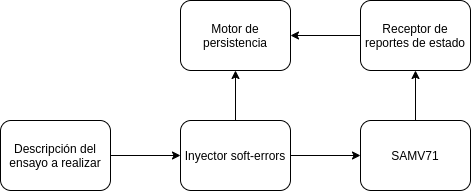
\includegraphics[width=0.7\textwidth]{./figuras/SISE.png}
	\caption{esquema general del sistema.}
	\label{fig:esqGral}
\end{figure}

El inyector de soft-errors deberá modificar los registros del microcontrolador SAMV71 según lo dispuesto en la descripción del ensayo.
En simultaneo, se debe persistir la modificación realizada.
Luego, se debe reportar el estado de funcionamiento del microcontrolador.
Finalmente, los reportes deben ser persistidos para su análisis.

\section{Funciones del producto}

El software aquí especificado brindará las siguientes funcionalidades:

\begin{itemize}
	\item Inyección de errores en todos los registros accesibles del microcontrolador SAMV71.
	\item Monitoreo del estado de funcionamiento del microcontrolador SAMV71.
	\item Persistencia de los soft-errors inyectados.
	\item Persistencia de los informes de estado de funcionamiento.
	\item Permitir escribir ensayos de evaluación.
	\item Presentación de resultados en histogramas que permitan un análisis estadístico.
\end{itemize}

\section{Características de los usuarios}

Los usuarios finales de este producto son ingenieros de desarrollo del INVAP.

\section{Restricciones}

Las restricciones del desarrollo del sistema son las siguientes:

\begin{itemize}
	\item Utilización de repositorio con control de versiones Gitlab.
	\item Documentación del código con Doxygen.
	\item Utilización exclusiva del lenguaje de programación Python.
\end{itemize}

\section{Suposiciones y dependencias}

La suposición principal es que se tendrá acceso irrestricto al microcontrolador SAMV71.

\section{Requisitos futuros}

N/A